%!TEX root = ../MainBody.tex

% 第二章
\chapter{需求分析}% 使用\cite{}命令引用数据库中文献
\section{系统陈述}
本系统主要分为两个模块:用户模块和管理员模块。用户登录/注册成功,可进行查阅、借书、还书、查看个人的已预约书籍列表和代还列表,以及物流地址等其他个人信息。管理员登录成功后,可查看预约列表,包含所有用户的远程预约信息,并根据预约信息查找馆内对应的纸质书籍,通过物流送达至各个用户所填写的物流地址,快递员将书籍送到用户手中。部分异常情况,例如书籍遗失,如果是用户本人遗失书籍,按照现行纸质书遗失规定办法处理;如
果是物流配送方遗失书籍,由配送方赔偿损失。
\section{用户使用场景}
\subsection{场景一:用户借书}
场景名:用户在登录web端,选择书籍,借书。

参与者实例:Tony,用户;Steve,图书管理员。

场景:

Tony登录“图书异地租借系统”web端,浏览书籍列表,选择一本《百年孤独》,点击进入详情页,查看书籍简介和馆藏信息,当前书籍状态为可借阅,点击下方`预约借书`按钮,等待管理员确认。

Steve登录“图书异地租借系统”web管理端,点击待借列表,看到Tony的借书请求,在图书馆中找到书籍,同时交付给物流公司,将物流号填写到管理端上。

Tony在web端上可以看见管理员填写的物流单号,据此查询物流状态。快递员将书籍派送至Tony手中,Tony终于可以阅读了。
\subsection{场景二:用户还书}
场景名:用户还书,在web端点击还书按钮,并填写物流单号。

参与者实例:Tony,用户;Steve,图书管理员。

场景:

Tony看完《百年孤独》,准备还书,将书籍交付物流公司,并点击web端,进入"我的-待还书籍",页面显示所有待还书列表,Tony点击《百年孤独》那一行,在弹出页面中填写物流单号,点击确定。

Steve收到快递员寄来的图书时,确认书籍完好无损,使用馆的还书机器进行还书扫描,扫描成功后该书籍的状态自动更新为"已归还"。

Tony的待还列表更新,《百年孤独》这一行没有已经不在该列表中。
\section{用例建模}
\begin{figure}[H] %H为当前位置,!hpb为忽略美学标准,hpbp为浮动图形
    \centering %图片居中
    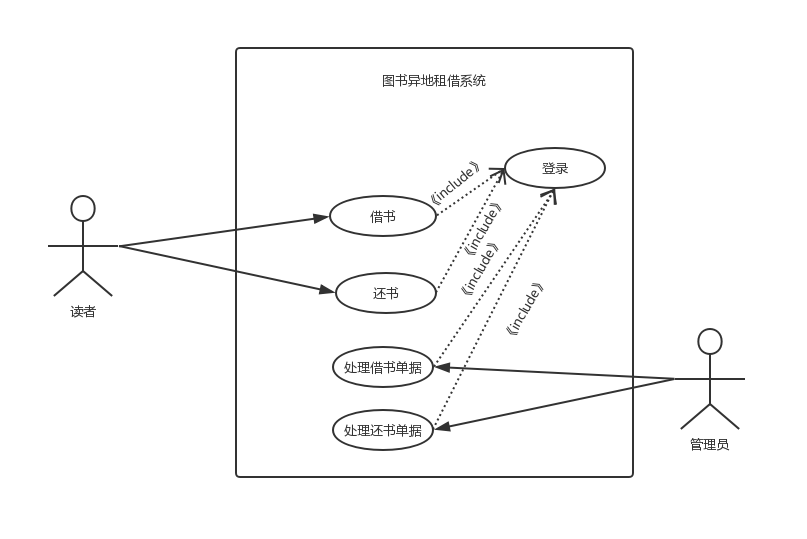
\includegraphics[width=0.7\textwidth]{./Chapters/images/example.png} %插入图片,[]中设置图片大小,{}中是图片文件名
    \caption{用例图} %最终文档中希望显示的图片标题
    \label{用例图} %用于文内引用的标签
\end{figure}
\begin{figure}[H] %H为当前位置,!hpb为忽略美学标准,hpbp为浮动图形
    \centering %图片居中
    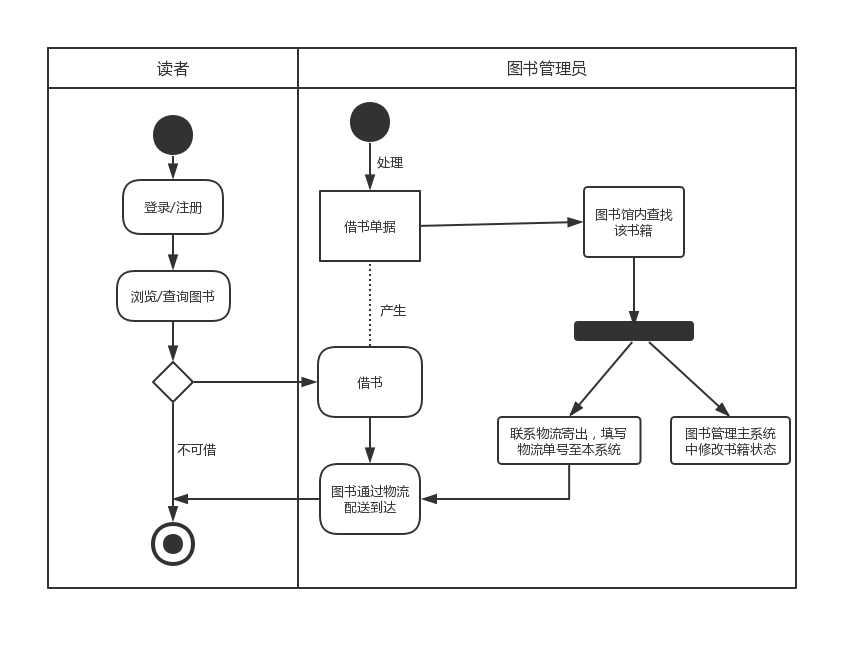
\includegraphics[width=0.7\textwidth]{./Chapters/images/activity.png} %插入图片,[]中设置图片大小,{}中是图片文件名
    \caption{活动图} %最终文档中希望显示的图片标题
    \label{活动图} %用于文内引用的标签
\end{figure}
\section{需求规约}
系统需求分为功能性需求和非功能性需求。功能需求可分为用户和管理员两大部分。对于用户来说,核心功能是在线预约书籍,书籍能够能通过物流方式送达。而管理员则主要是处理用户的预约请求,将书籍交付物流。
\subsection{功能性需求}
\subsubsection{用户相关的功能需求}
\begin{itemize}
    \item 登录/注册,登录的账号密码与借书卡的账号密码一致,读者注册于图书管理主 系统一致,需要到馆内注册借书卡,注册成功后,通过借书卡的账号/密码登录本系统。
    \item 图书列表展示,以图文卡片列表的方式展示图书馆馆藏书籍,卡片中包含书籍 的作者、出版社、简介等基本信息和借书条码号、可借数量及馆藏总数量等,可 借数量大于 0 时,读者可以点击预约按钮进行预约借阅。
    \item 借还书操作,在系统中的书籍列表和已预约列表中,可进行预约借书/取消预约 操作。在待还列表中可点击还书按钮,申请还书。
    \item 个人信息,包含物流地址信息、已预约书籍列表、待还列表等个人信息。
\end{itemize}
\begin{table}[hp]
    \centering
    \caption{用户登录}
	\begin{tabular*}{\textwidth}{p{0.25\textwidth}|p{0.7\textwidth}}
    \hline
    用例名称    & 用户登录                                                                                                                             \\ \hline
    用例描述    & 用户通过账号密码登录本系统的整个流程                                                                                                               \\ \hline
    执行者     & 用户                                                                                                                               \\ \hline
    前置条件    & 该用户拥有图书馆的借书卡,并知道借书卡的账号和密码                                                                                                        \\ \hline
    后置条件    & 生成有效期为7天的唯一登录token                                                                                                                             \\ \hline
    主事件流描述  & \begin{enumerate} 
            \item 用户在未登录(未登录规则参见业务规则a)的情况下,访问本系统的任意界面,系统自动跳转至登录界面;
            \item 用户输入持有借书卡的账号和密码,系统校验输入的账号和密码,应用业务规则b,若校验失败,执行异常过程2.1.1;若校验成功,系统自动跳转至主界面。
        \end{enumerate} \\ \hline
    分支事件流描述 & ~                                                                                                                                \\ \hline
    异常事件流描述 & 2.1.1 若不存在该账号,则系统提示该账号不存在;若账号和密码不匹配,则系统提示账号密码不匹配,返回2                                                                             \\ \hline
    业务规则    & a. 未登录状态可由2种情况判定:1. 用户第一次登录;2.  用户之前登录过,但登录token已失效 b. 先查询系统中是否存在该账号,不存在则校验失败,存在则校验账号和加密后的密钥是否与数据库中存储的数据匹配,不匹配则校验失败,匹配则校验成功.    \\ \hline
    涉及的业务实体 & 借书卡账号、密码                                                           \\ \hline
\end{tabular*}
\end{table}
\begin{figure}[H]
    \centering  %图片全局居中
    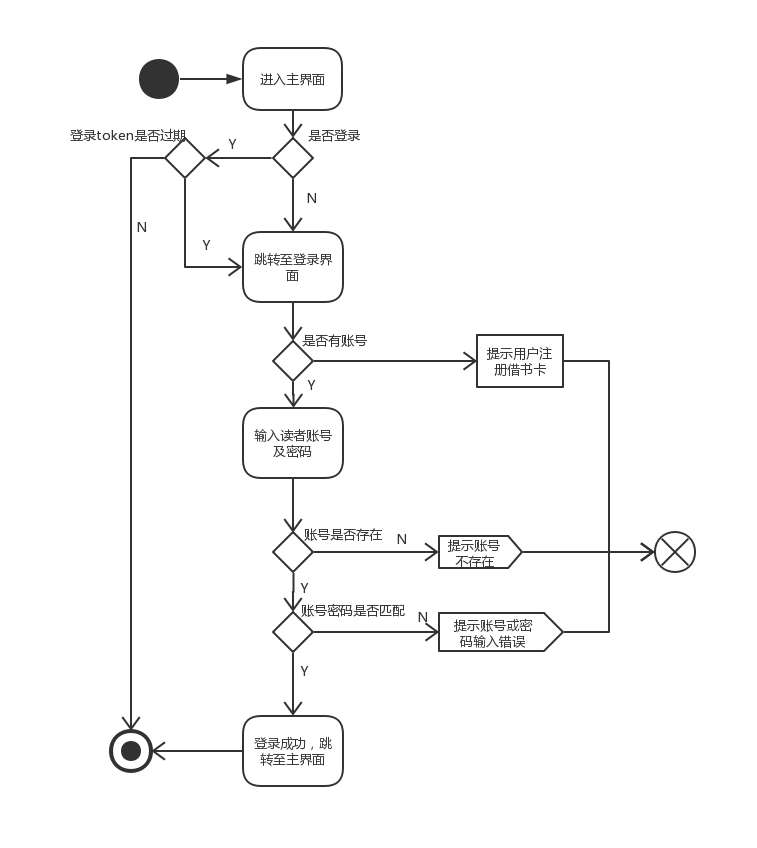
\includegraphics[width=0.45\textwidth]{./Chapters/images/activity_login.png}
    \caption{登录活动图}
    \label{登录活动图}
\end{figure}
%图书列表展示:
\begin{table}[hp]
    \centering
    \caption{浏览图书列表}
	\begin{tabular*}{\textwidth}{p{0.25\textwidth}|p{0.7\textwidth}}
    \hline
    用例名称    & 浏览图书列表    \\ \hline
    用例描述    & 用户进入主界面,浏览图书列表,查看图书信息    \\ \hline
    执行者     & 用户         \\ \hline
    前置条件    & 用户已成功登录本系统   \\ \hline
    后置条件    & ~     \\ \hline
    主事件流描述  & \begin{enumerate} 
            \item 用户进入主界面,系统显示书籍列表,每个列表项展示书籍封面、书名、可借数量、馆藏数量、预约按钮、详情按钮
            \item 用户点击借书,若书籍可借数量为0,应用业务规则a,否则执行分支过程2.1.1,若用户点击详情,执行分支过程2.2.1
        \end{enumerate} \\ \hline
    分支事件流描述 & \begin{itemize} 
        \item[2.1.1] 弹出二次确认框,点击确认则请求预约借书,取消则用例终止
        \item[2.2.1] 详情按钮上方弹出气泡,气泡中显示书籍简介信息
    \end{itemize}     \\ \hline
    异常事件流描述 & ~  \\ \hline   
    业务规则    &  a. 若预约按钮不可点击  \\ \hline
    涉及的业务实体 & 图书      \\ \hline
\end{tabular*}
\end{table}
% 借书操作
\begin{table}[hp]
    \centering
    \caption{借书操作}
	\begin{tabular*}{\textwidth}{p{0.25\textwidth}|p{0.7\textwidth}}
    \hline
    用例名称    & 借书操作    \\ \hline
    用例描述    & 用户进入主界面,浏览图书列表,进行借书操作    \\ \hline
    执行者     & 用户         \\ \hline
    前置条件    & 1. 用户已成功登录本系统;2. 所选择的图书可借数量大于0  
     \\ \hline
    后置条件    & 1. 系统生成预约记;2. 管理员可查看该预约记录;3. 提交预约申请后可撤销  
    \\ \hline
    主事件流描述  & \begin{enumerate} 
            \item 用户浏览图书列表,点击某本书左下角的借书按钮,应用业务规则a,若该本书的可借数量为0,执行1.1.1,若可借数量大于0,执行2,点击预约列表,执行4
            \item 用户点击借书按钮后,系统弹出二次确认框,点击取消,用例结束;点击确认,系统发起借书请求,执行3
            \item 若系统请求成功,借书按钮的文案变为“已预约”,点击按钮,执行3.1.1
            \item 用户点击“预约列表”之后,系统展示所有已预约书籍列表,点击取消按钮,执行3.1.1
        \end{enumerate} \\ \hline
    分支事件流描述 & \begin{itemize}
        \item[1.1.1]  按钮不可点击,用例结束
        \item[3.1.1] 弹出"是否取消预约"的二次确认框,确认则系统发起取消预约请求,用例结束      
    \end{itemize} \\ \hline
    业务规则    &  a. 若该本书的可借数量大于0,则借书按钮可点击;若该本书的可借数量为0,则按钮为不可点击状态  \\ \hline
    涉及的业务实体 & ~     \\ \hline
\end{tabular*}
\end{table}
%还书操作
\begin{table}[hp]
    \centering
    \caption{还书操作}
    \begin{tabular*}{\textwidth}{p{0.25\textwidth}|p{0.7\textwidth}}
        \hline
    用例描述    & 用户在系统上申请还书,并交付物流或到馆还书的流程。    \\ \hline
    执行者     & 用户      \\ \hline
    前置条件    & 1.用户将书籍交付物流公司,并获取到物流单号    2.用户成功登录系统,待还列表中有该待还书籍   \\ \hline
    后置条件    & 1. 用户本人未造成书籍为损坏或遗失     2.物流配送过程中,书籍未损坏或遗失  3.管理员更新书籍为已还状态    \\ \hline
    主事件流描述  & \begin{enumerate} 
            \item 用户进入系统主界面,点击待还列表,找到待还图书所在的具体行,若未申请过还书,执行2;若已申请过还书,执行3
            \item 点击"我要还书"按钮,页面显示弹出框,在弹出框内填写物流单号,点击确认,执行分支过程2.1.1
            \item 列表项显示上次成功提交的物流单号,点击"修改物流"按钮,页面显示弹出框,在弹出框中修改物流信息,点击确认,执行分支过程2.1.1
            \item 物流公司配送书籍至图书馆,若书籍在配送过程中损坏或遗失,执行异常过程4.1.1
        \end{enumerate} \\ \hline
    分支事件流描述 & 2.1.1 系统提交表单,若提交成功,生成历史单号;若提交失败,系统提示提交失败,页面停留在表单编辑页    \\ \hline
    异常事件流描述 & 4.1.1 书籍损坏,图书管理员收到图书后,应用业务规则a,按照图书馆现行书籍损坏赔偿制度向物流公司或用户索赔;书籍遗失,管理员按照现行图书遗失赔偿制度向物流公司索赔 \\ \hline                                                                            \\ \hline
    业务规则    &  a. 书籍损坏,读者上传照片等凭证,须管理员确认读者本人未损坏书籍,否则由读者赔偿。 \\ \hline
    涉及的业务实体 & 图书、物流单号    \\ \hline
\end{tabular*}
\end{table}
\begin{figure}[H]
    \centering  %图片全局居中
    \subfigure[借书活动图]{
    \label{借书活动图}
    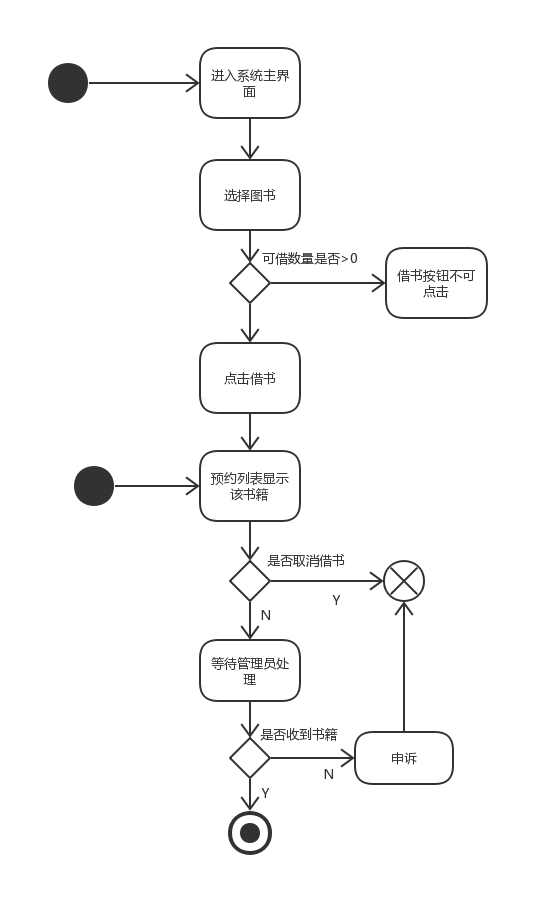
\includegraphics[width=0.45\textwidth]{./Chapters/images/activity_borrow.png}}
    \subfigure[还书活动图]{
    \label{还书活动图}
    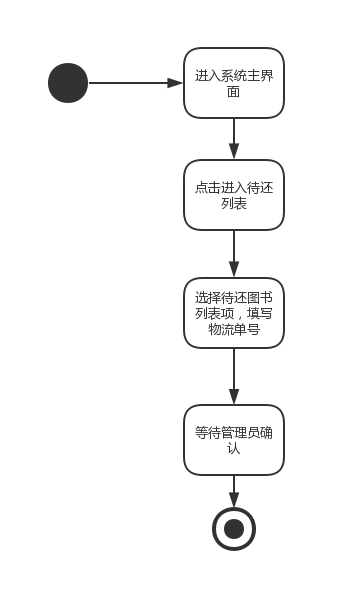
\includegraphics[width=0.45\textwidth]{./Chapters/images/activity_back.png}}
    \caption{借还书活动图}
    \label{借还书活动图}
\end{figure}
\subsubsection{管理员相关的功能需求}
\begin{itemize}
    \item 登录,与图书管理主系统账号密码一致,由于管理员的角色特殊性,本系统不 提供注册功能,只能根据已有账号密码进行登录操作。
    \item 处理书籍预约,列表的每一项展示书籍名称、借书条码号、读者 ID、读者姓名、 预约时间等信息和还书状态修改按钮。
\end{itemize}
\begin{table}[hp]
    \centering
    \caption{处理借书单据}
	\begin{tabular*}{\textwidth}{p{0.25\textwidth}|p{0.7\textwidth}}
    \hline
    用例名称    & 管理员处理借书单据    \\ \hline
    用例描述    & 管理员登录系统,查看图书预约列表,在馆内找到实体书并交付物流的整个流程   \\ \hline
    执行者     & 图书管理员       \\ \hline
    前置条件    & 1.用户申请预约书籍,预约列表显示读者的预约信息  \\ \hline
    后置条件    & 1. 书籍状态更新为已借出    \\ \hline
    主事件流描述  & \begin{enumerate} 
            \item {[查看预约列表]}管理员登录系统,查看读者预约列表,列表展示应用业务规则a,若管理员在搜索框中输入关键字,执行分支流程1.1.1,否则依次查看列表项的预约信息,执行2
            \item {[馆内获取实体书]}管理员根据预约信息上的书籍条码号,获取书籍馆藏位置,在馆内查找并取得书籍,若未查找到书籍,执行异常过程2.1.1
            \item {[物流交付]}管理员将书籍交付物流,并在预约列表对应项中填写物流单号,应用业务规则b
        \end{enumerate} \\ \hline
    分支事件流描述 & 1.1.1 关键字可为书名、书籍条码号、读者ID,系统根据管理员输入的关键字进行查询,返回筛选后的数据    \\ \hline
    异常事件流描述 & 2.1.1 管理员通知读者,该书籍目前不可借,读者取消预约,用例结束 \\ \hline                                                                            \\ \hline
    业务规则    &  \begin{enumerate}[label=\alph*]
        \item 列表默认按照时间由远及近、物流地址的顺序、读者名称的字母顺序展示
        \item 书籍状态为已借出,读者在待还列表中可查看寄出的物流单号    
    \end{enumerate} \\ \hline
    涉及的业务实体 & 图书、物流单号    \\ \hline
\end{tabular*}
\end{table}
\begin{table}[p]
    \centering
    \caption{处理还书单据}
	\begin{tabular*}{\textwidth}{p{0.25\textwidth}|p{0.7\textwidth}}
    \hline
    用例名称    & 处理还书单据   \\ \hline
    用例描述    & 管理员检查书籍是否损坏,损坏则理赔,未损坏则将图书归还图书   \\ \hline
    执行者     & 图书管理员        \\ \hline
    前置条件    & 1.书籍未遗失或损坏        2. 异地借出的图书通过物流送达至图书馆    \\ \hline
    后置条件    & 1. 书籍状态更新为"可借"       2. 将图书放置到指定的馆藏位置  \\ \hline
    主事件流描述  & \begin{enumerate} 
            \item  {[收到图书]} 物流公司将书籍配送到图书馆,若书籍遗失,执行异常过程1.1.1,管理员检查书籍,若损坏,执行异常过程1.2.1,若管理员登录系统,查看待还列表,执行分支流程1.1.1
            \item 管理员执行分支过程2.1.1,将书籍状态修改为"可借",若管理员登录系统并常看待还列表,执行分支过程2.2.1
        \end{enumerate} \\ \hline
    分支事件流描述 & \begin{itemize}
        \item[1.1.1] 待还列表展示通过本系统借出的所有书籍,若该书籍已被交付物流,系统展示物流单号
        \item[2.1.1] 管理员可通过图书馆的还书扫描仪、扫码枪或手动输入书籍条码号,进行还书操作
        \item[2.2.1] 待还列表不再展示该书籍 
    \end{itemize}    \\ \hline
    异常事件流描述 & \begin{itemize}
        \item[1.1.1] 书籍遗失,联系物流公司索赔
        \item[1.2.1] 书籍损坏,管理员确认是读者损坏还是物流公司损坏,进行索赔
    \end{itemize}                                                                              \\ \hline
    业务规则    &  a. 列表默认按照时间由远及近、物流地址的顺序、读者名称的字母顺序展示。   b. 书籍状态为已借出,读者在待还列表中可查看寄出的物流单号  \\ \hline
    涉及的业务实体 & 图书     \\ \hline
\end{tabular*}
\end{table}
\begin{figure}[H]
    \centering  %图片全局居中
    \subfigure[处理借书活动图]{
    \label{处理借书活动图}
    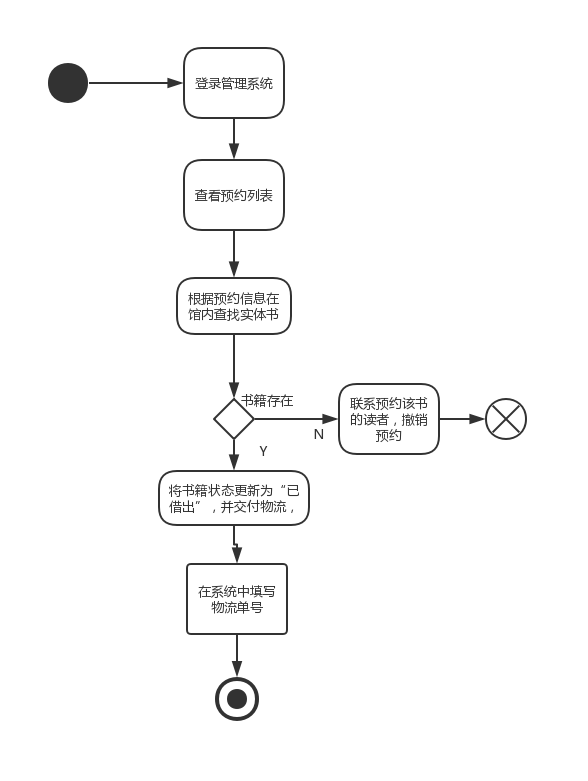
\includegraphics[width=0.45\textwidth]{./Chapters/images/activity_handle_borrow.png}}
    \subfigure[处理还书活动图]{
    \label{处理还书活动图}
    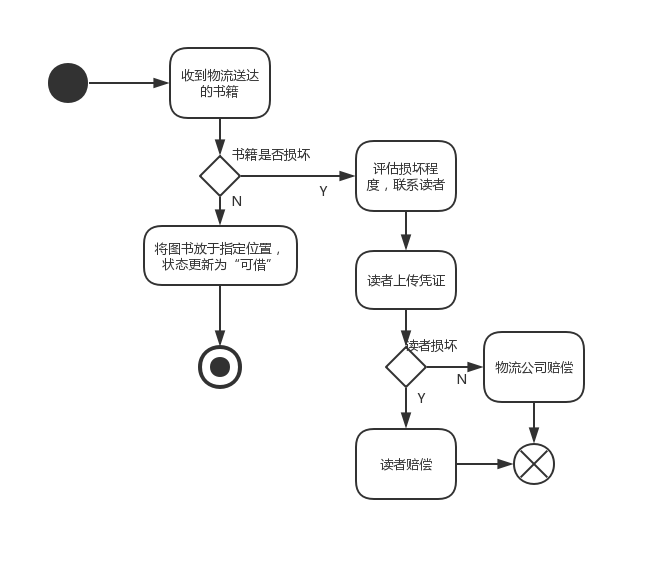
\includegraphics[width=0.45\textwidth]{./Chapters/images/activity_handle_back.png}}
    \caption{处理借还书活动图}
    \label{处理借还书活动图}
\end{figure}
\subsection{业务规则}
\begin{itemize}
    \item 借还书时间规定,书籍的借出时间为管理员修改书籍为"已借出"的具体时间,归还时间为管理员修改书籍状态为"已归还",或用户亲自到馆归还的具体时间。其中,物流配送时间算借书时间内。以四川大学图书馆为例,用户借书期限为30天,如果某用户通过本系统异地借阅书籍,实际取得书籍的时间是小于30天的。    
\end{itemize}
\subsection{非功能性需求}
\begin{itemize}
    \item 系统稳定性。由于系统具有展示、预约,还书、记录物流的功能。用户会在页面间来回跳转,点击。应该设计好页面的路由规则,预约请求的幂等性,维护预约事件列表,处理好事件循环,保证系统在网络异常或暴力操作时的数据准确性和系统稳定性。
    \item 系统安全性。由于本系统基于web端访问,应处理好XSS、CSRF、SSRF、DDoS等安全攻击,系统采用登录保护,没有借书卡的用户不允许登录,同时进行token校验,refer验证等方式,一定程度上保护了个人隐私,提高用户的信息安全性。
    \item 交互友好性。本系统为用户提供友好美观的图文操作页面,采用流式布局,分析用户操作流程,优化界面布局和操作步骤,提供优质的用户体验。同时,在书籍即将超期时推送消息,提醒用户进行及时还书。
\end{itemize}
